% Add `ngerman` to documentclass for German docs
\documentclass[12pt, a4paper]{article}
\usepackage{a4wide}
\usepackage{setspace}
\usepackage{csquotes}
\usepackage[utf8]{inputenc}

\usepackage{url}
\usepackage[hidelinks]{hyperref}
\usepackage{minted}
\usemintedstyle{perldoc}

% inline code
\newcommand{\code}[1]{\texttt{#1}}

% Uncomment for German
%\usepackage[ngerman]{babel}

% For generating template dummy text
\usepackage{lipsum}

\usepackage{myColors}
\usepackage{myFooter}
\usepackage{myTitle}

% Libraries outside of template
\usepackage[T1]{fontenc}
\usepackage{upquote}
\AtBeginDocument{%
    \def\PYZsq{\textquotesingle}%
}

%%%%%%%%%%%%%%%%%%%%%%%%%%%%%%%%%%%%%%%%%%%%%%%%%%%%%%%%%%%%%%%%%%%%%%%

\project{CS 432 Web Science}
\author{Derek Goddeau}
\title{Assignment Four}
\supervisor{Michael L. Nelson}

\doublespace
\pagestyle{hacker}

\begin{document}
\maketitle

\newpage



%%%%%%%%%%%%
% Facebook %
%%%%%%%%%%%%
\section{Facebook Friendship Paradox}

In order to represent the data from the GraphML file I used the R \code{igraph}
library. After reading it from the file I created a dataframe with all of the
vertex attributes from which I subset only the needed data, names and friend counts.
The \code{na.omit()} call removes $11$ friends with no friend data from the dataset.

\begin{minipage}{\linewidth} % prevent splitting between pages
\vspace{2em}
\begin{minted}[fontfamily=tt]{r}
library(igraph)
g <- read_graph('../data/mln.graphml', format = c('graphml'))
df <- vertex_attr(g)

df.self <- data.frame(friend_count = 234, name = 'Michael L. Nelson')
df.friends <- data.frame(friend_count = df$friend_count, name = df$name)
df.all <- rbind(df.friends, df.self)
df.sorted <- na.omit(df.all[with(df.all, order(friend_count)), ])
\end{minted}
\vspace{2em}
\end{minipage}

\noindent
The R \code{summary()} and \code{sd()} methods were used to calculate the
mean, standard deviation, and median values.

\vspace{2em}
\begin{table}[h]
    \centering
    \begin{tabular}{|c|c|c|}
        \hline
        \textbf{Mean} & \textbf{Median} & \textbf{Standard Deviation} \\ \hline
        359           & 267             & 372                         \\ \hline
    \end{tabular}
    \caption{Facebook Friend Statistics}
\end{table}
\vspace{2em}

\noindent
As shown in figure~\ref{fig:friends} on page~\pageref{fig:friends} the
friendship paradox holds with both the median and mean. There are a small
amount of outliers that skew the data slightly but not enough to question
the outcome.

\begin{figure}[p]
    \centering
    \href{http://datenstrom.gitlab.io/cs532-s17/notebooks/friends.html}{
    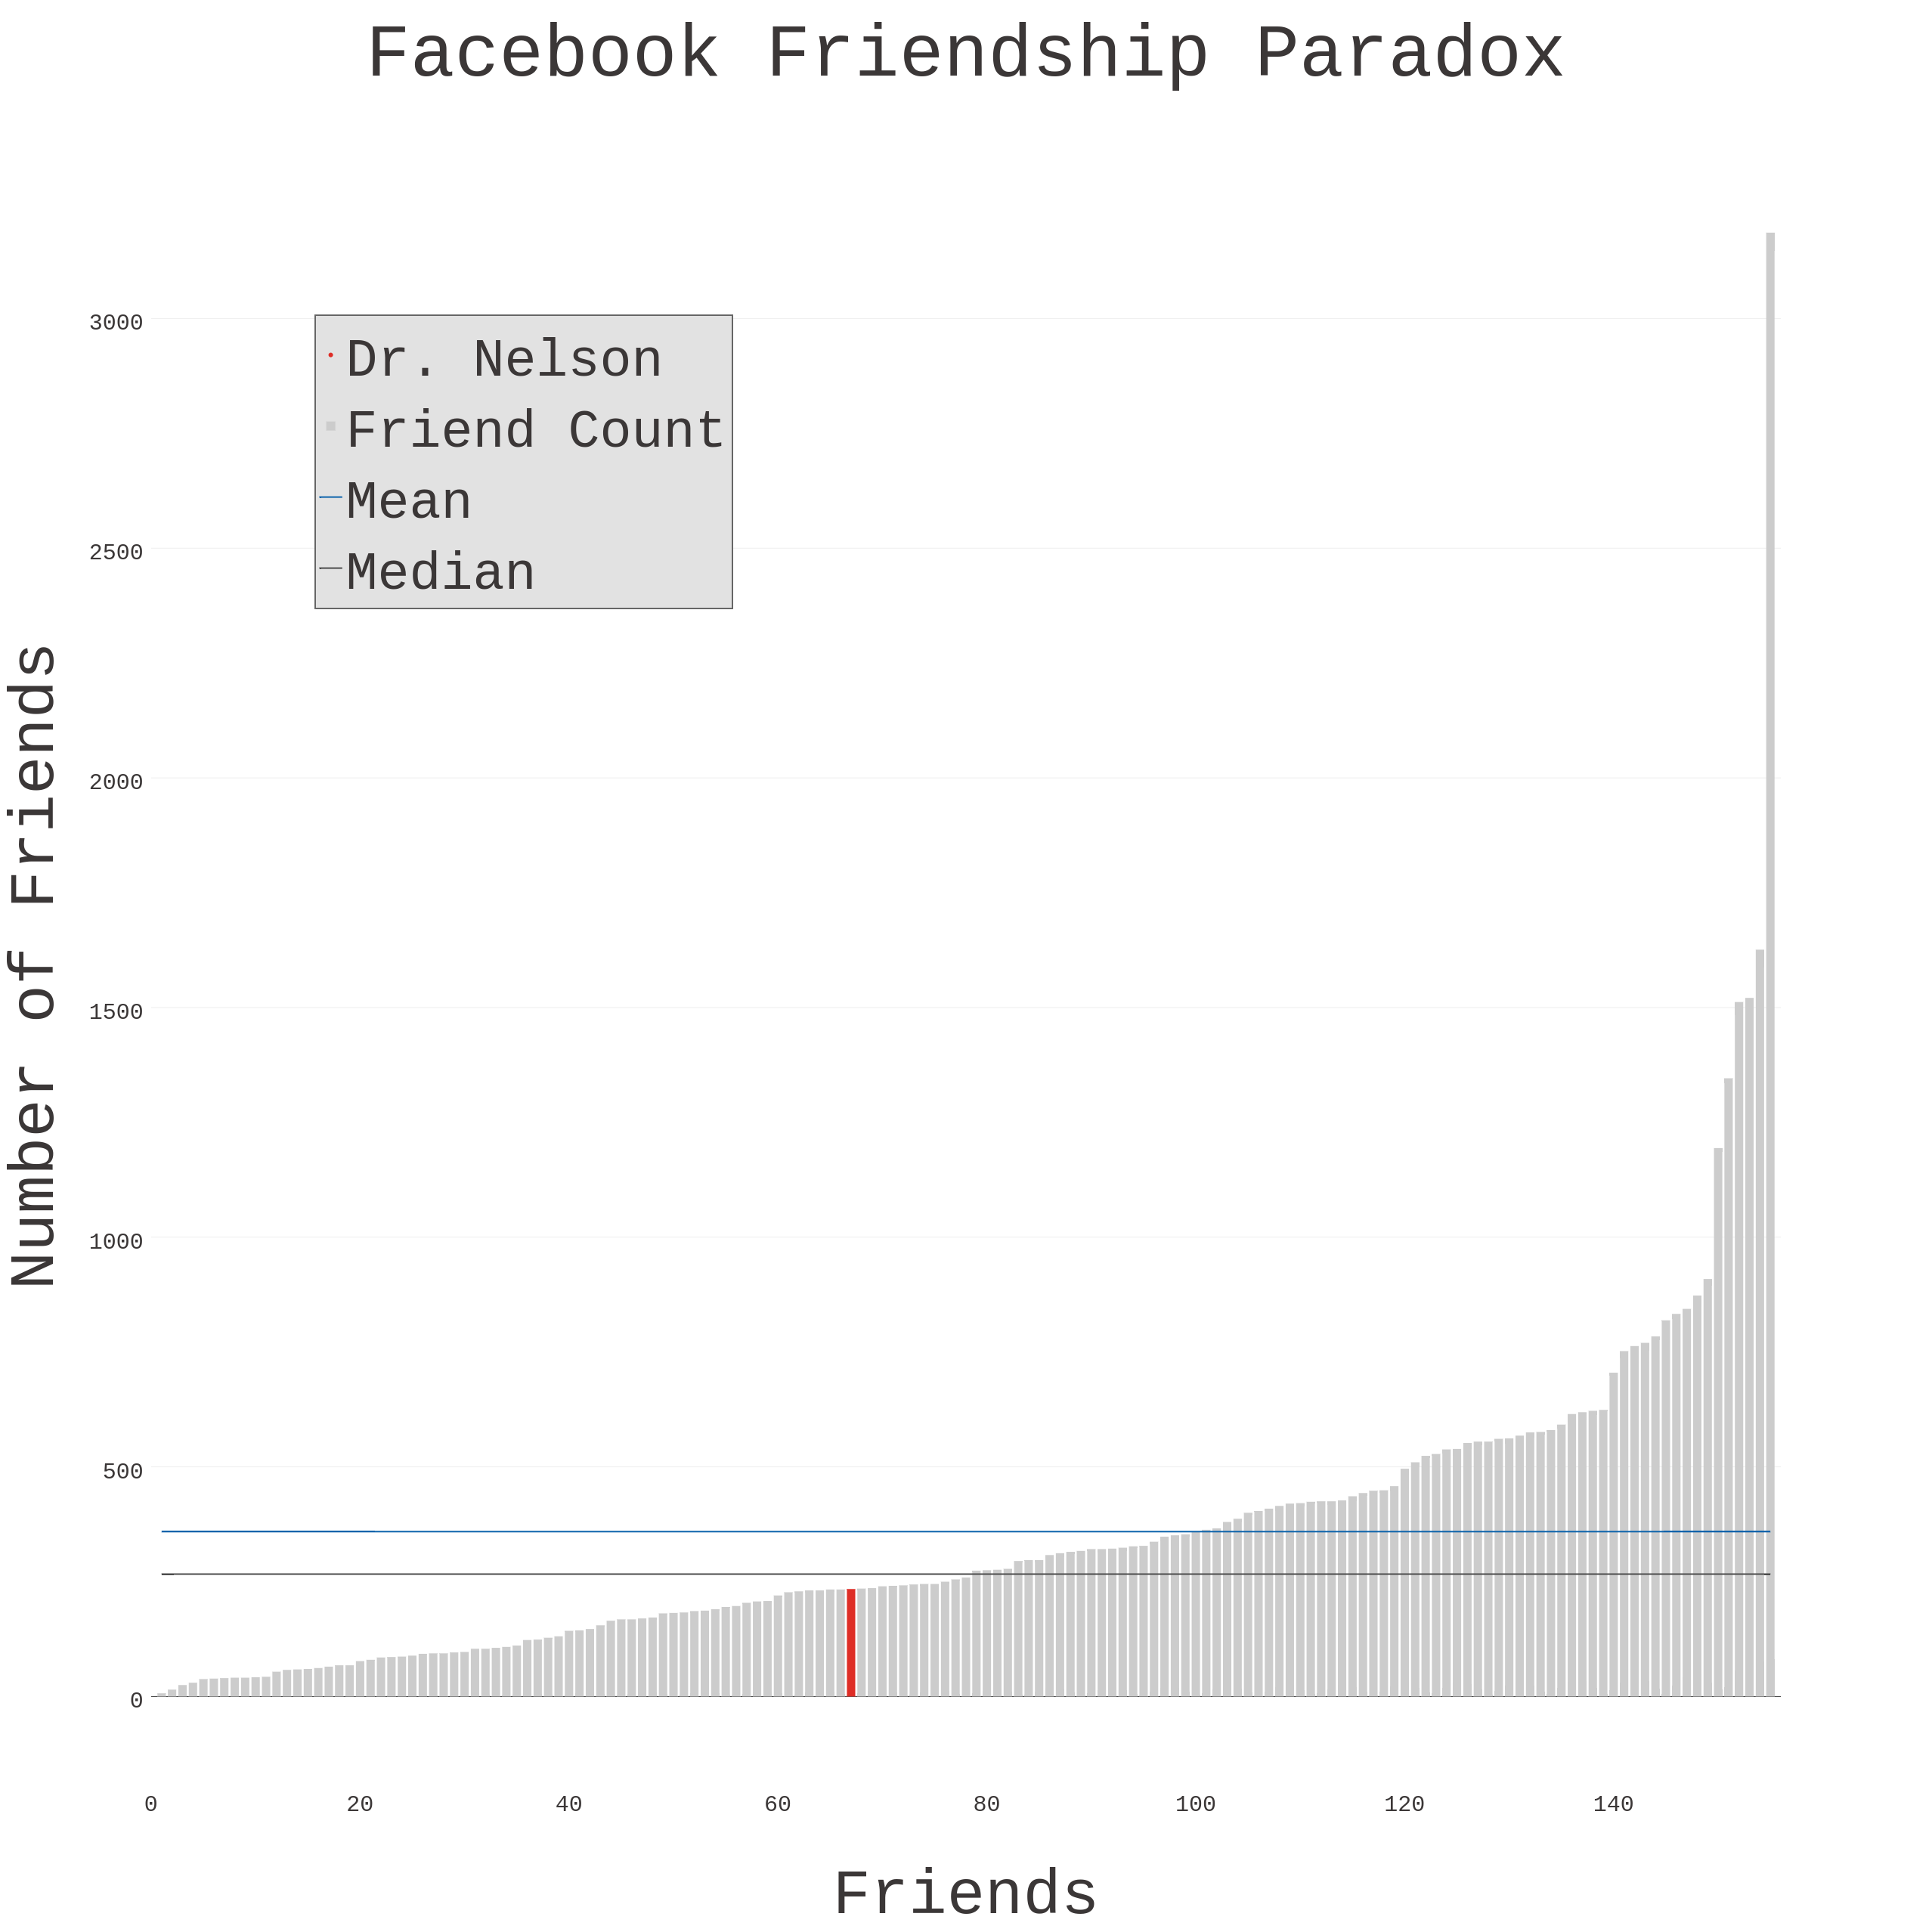
\includegraphics[width=\textwidth]{dia/friends.png}
    }
    \caption{Dr. Nelson's Facebook Friends}
    \label{fig:friends}
\end{figure}


%%%%%%%%%%%
% Twitter %
%%%%%%%%%%%
\section{Twitter Friendship Paradox}

To get the twitter followers I used Python but this time \code{python-twitter}
instead of \code{tweepy}. This allowed for much simpler fetching of the followers 
as shown below it is reduced to a one liner after authenticating,
but provides no way to get the data out of their \code{User} object, so I wrote
just the data I needed to a CSV file for R to read in.

\begin{minipage}{\linewidth} % prevent splitting between pages
\vspace{2em}
\begin{minted}[fontfamily=tt]{python}
    followers = self.api.GetFollowers(self.username)
\end{minted}
\vspace{2em}
\end{minipage}

\noindent
From there it is the same exact process as with the Facebook data in R.
Again I used \code{summary()} and \code{sd()} to get the statistics.

\vspace{2em}
\begin{table}[h]
    \centering
    \begin{tabular}{|c|c|c|}
        \hline
        \textbf{Mean} & \textbf{Median} & \textbf{Standard Deviation} \\ \hline
        1508          & 310             & 10143                       \\ \hline
    \end{tabular}
    \caption{Twitter Follower Statistics}
\end{table}
\vspace{2em}

\noindent
With this data, as shown in figure~\ref{fig:followers-full} on
page~\pageref{fig:followers-full} there are some extreme
outliers which will skew the average and in fact the average is
quite a bit larger than the mean. In figure~\ref{fig:followers-half}
on page~\pageref{fig:followers-half} Dr. Nelson's follower count is
well above the median but also well below the average.
In this case by the mean value the friendship paradox holds, but
the median is a better value to judge the quality and
therefore the friendship paradox does not hold. With clever use
of statistics and graphs either argument could be made about the
model.


\begin{figure}[p]
    \centering
    \href{http://datenstrom.gitlab.io/cs532-s17/notebooks/followers.html}{
    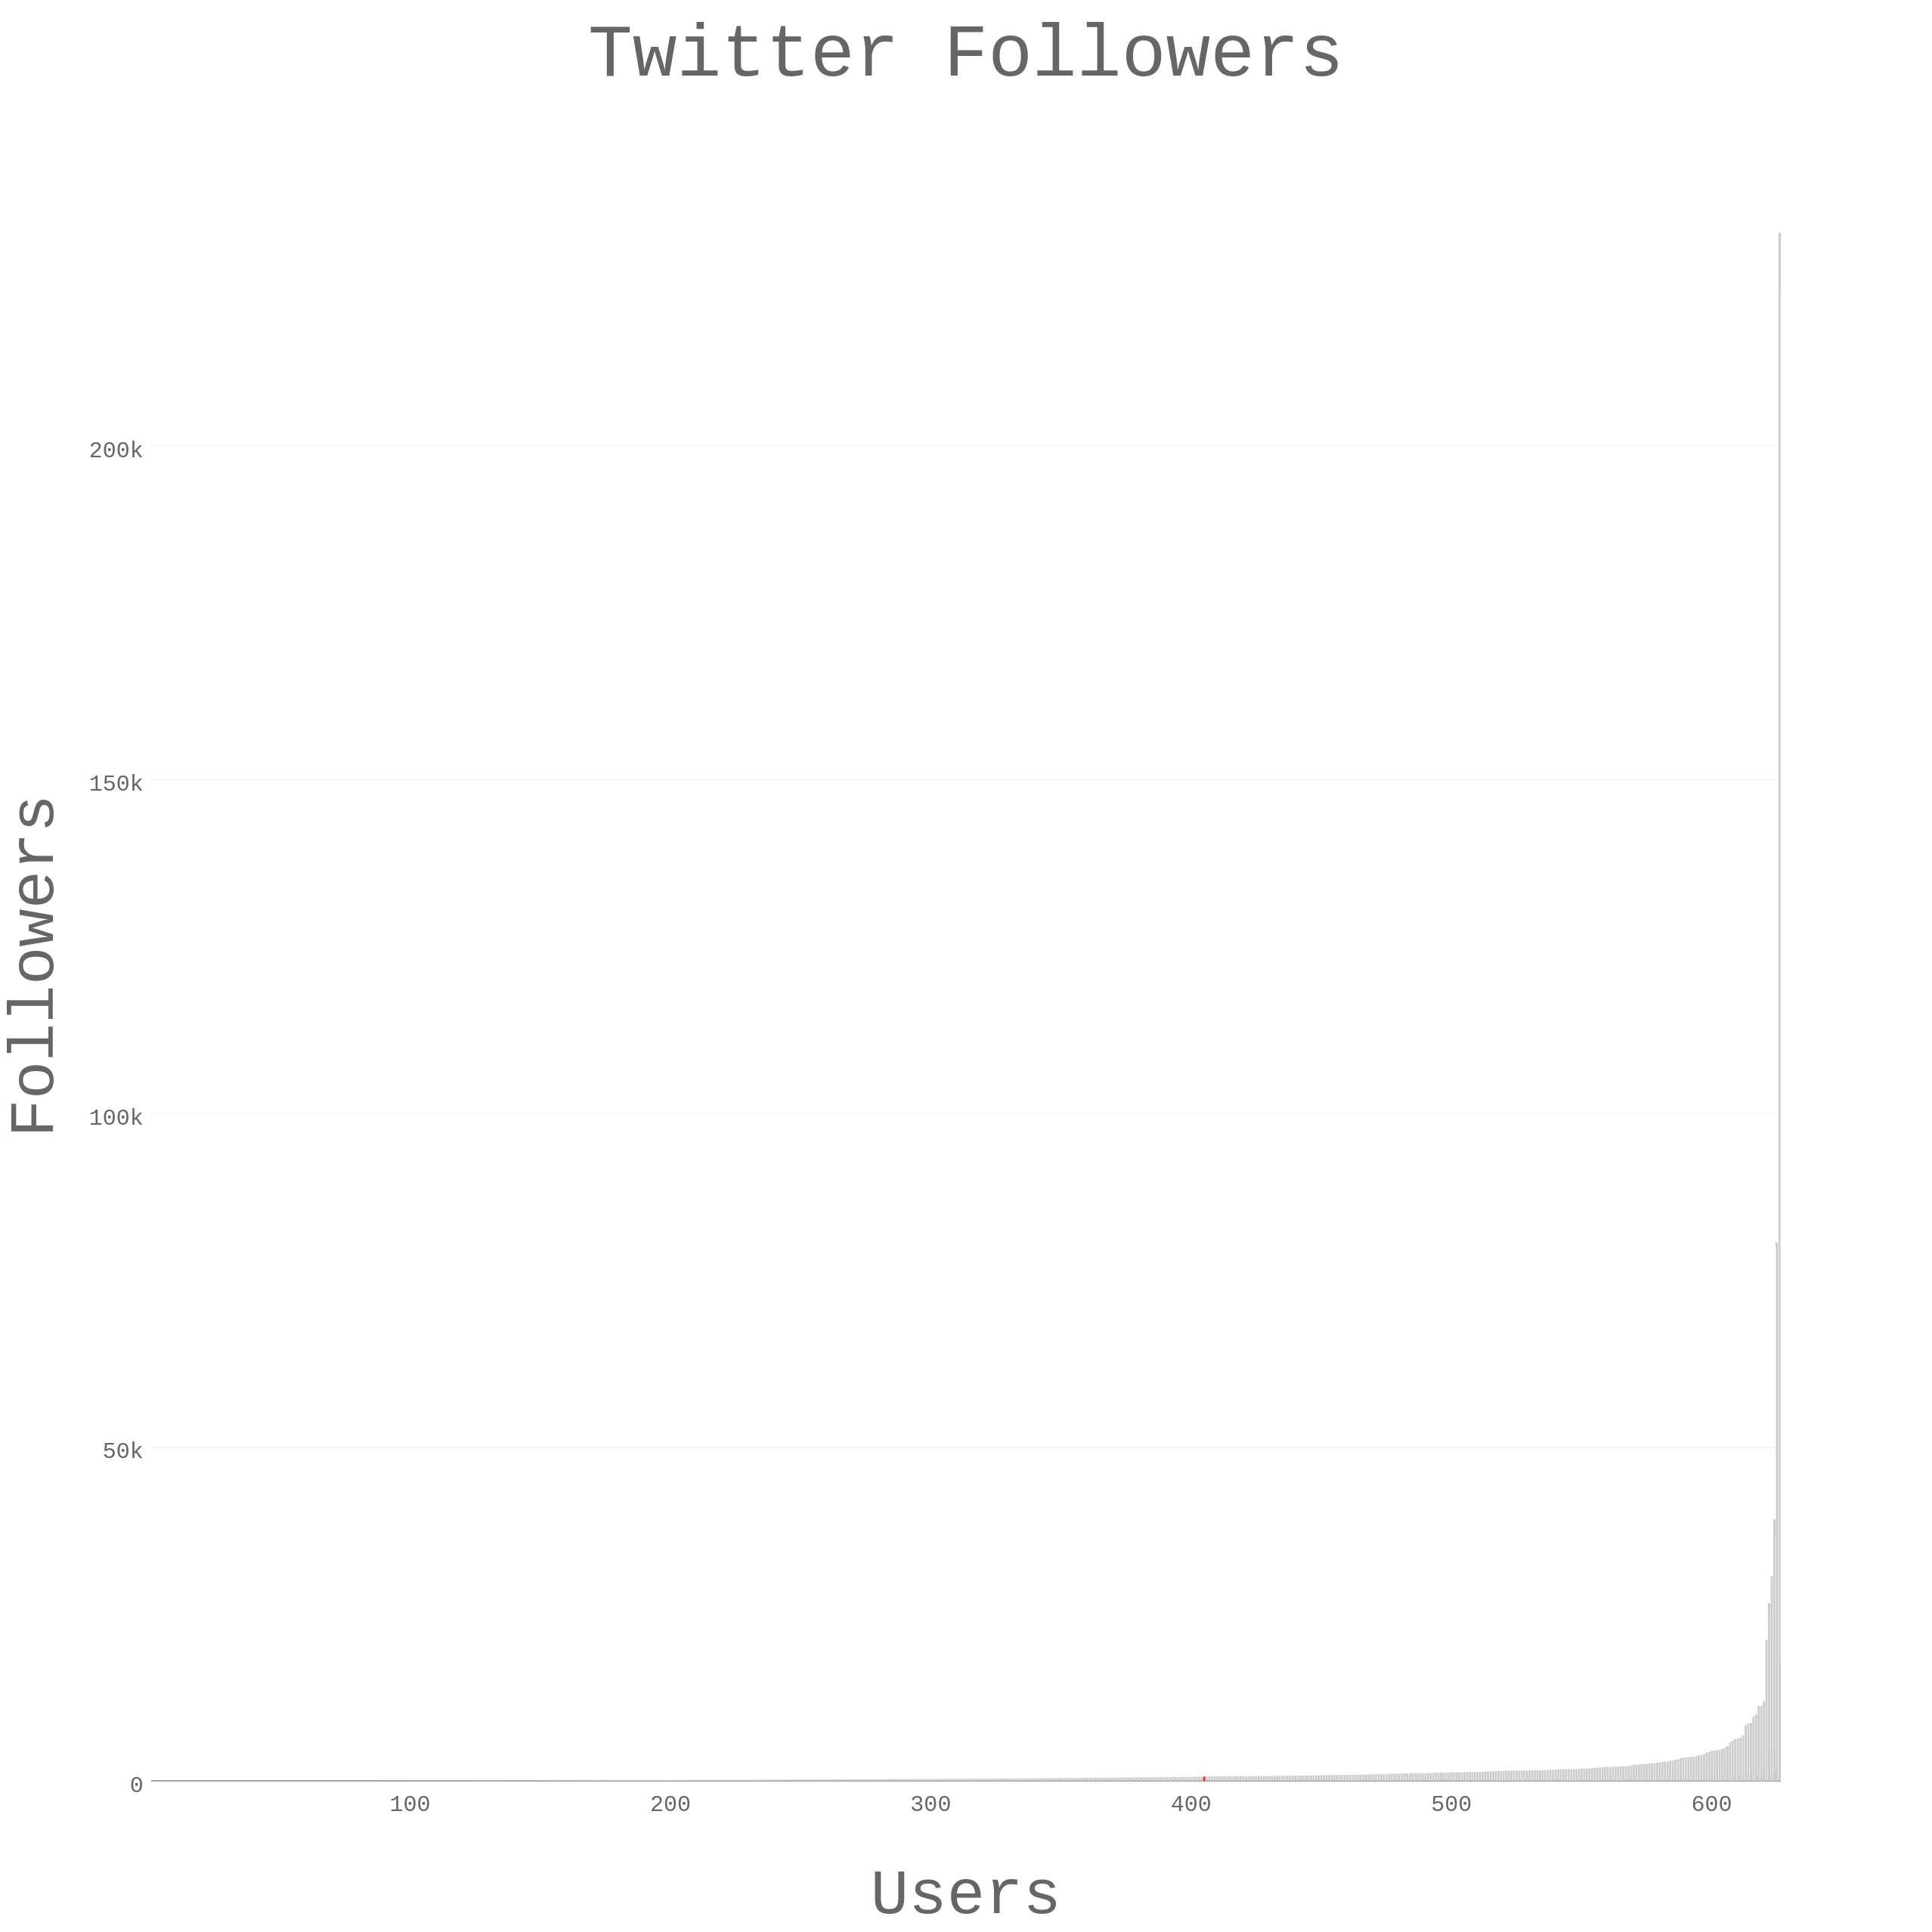
\includegraphics[width=\textwidth]{dia/followers_full.png}
    }
    \caption{Dr. Nelson's twitter followers}
    \label{fig:followers-full}
\end{figure}

\begin{figure}[p]
    \centering
    \href{http://datenstrom.gitlab.io/cs532-s17/notebooks/followers.html}{
    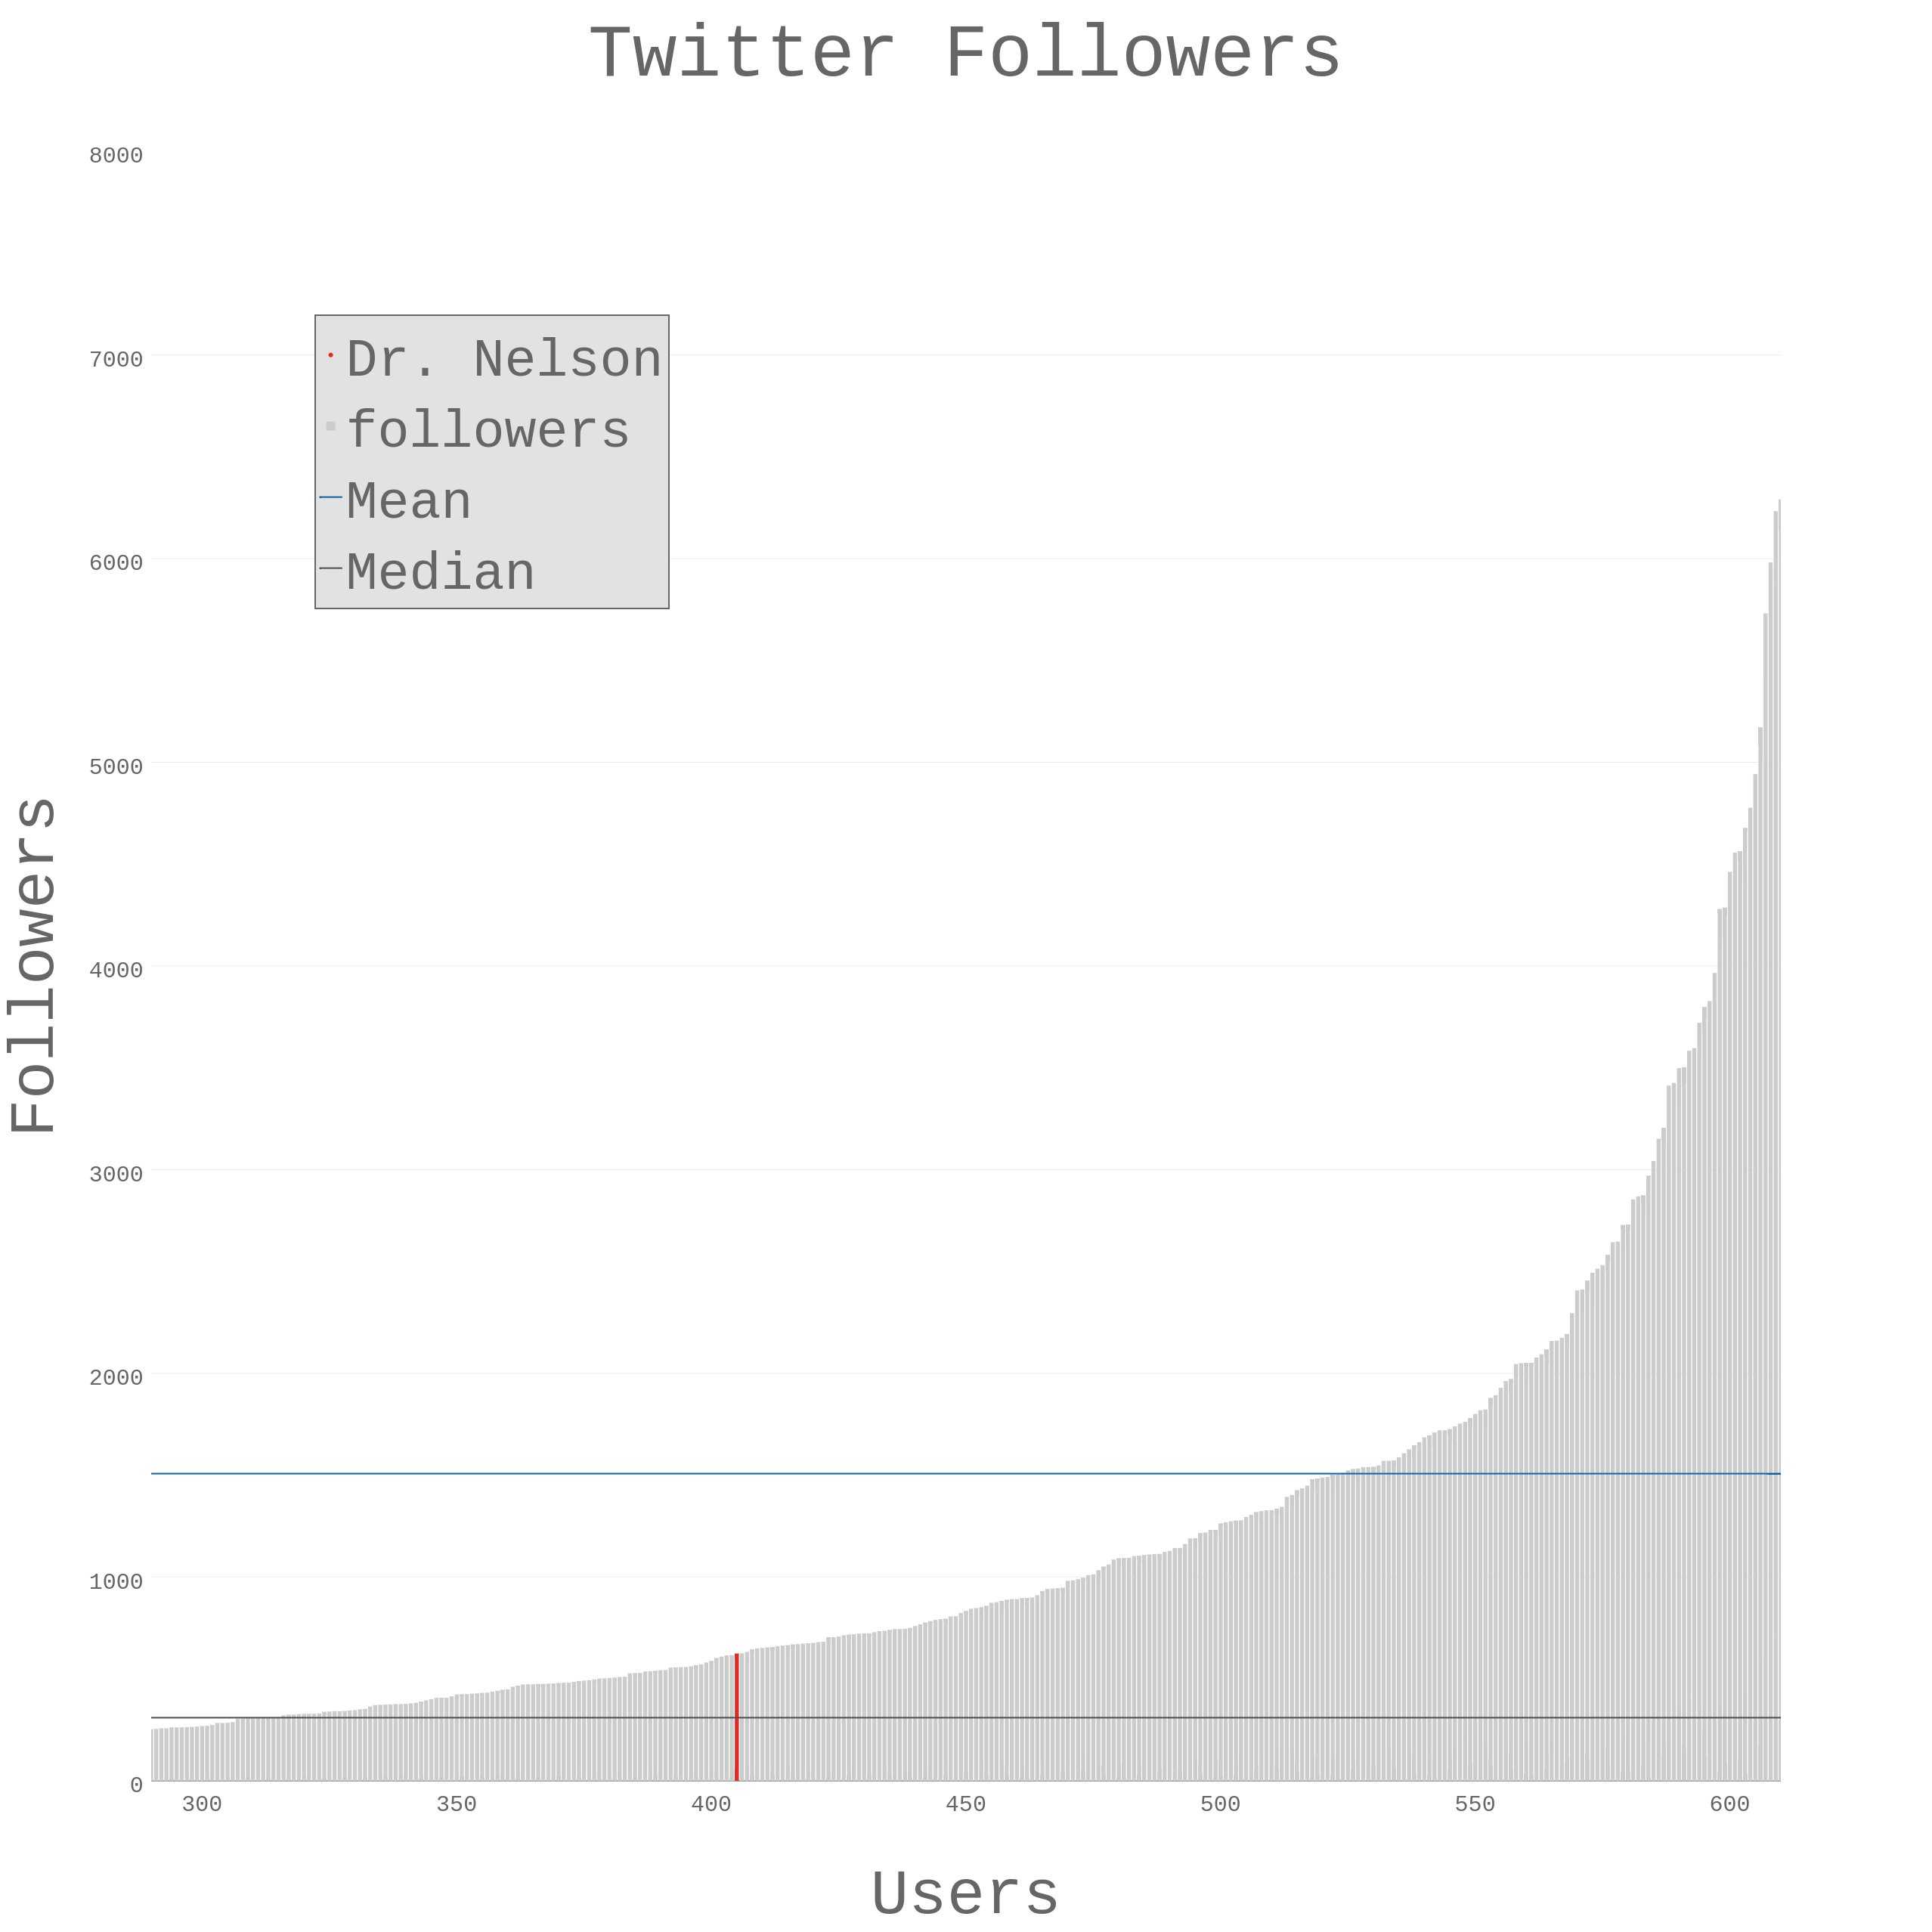
\includegraphics[width=\textwidth]{dia/followers_half.png}
    }
    \label{fig:followers-half}
    \caption{Dr. Nelson's twitter followers}
\end{figure}

\end{document}
